\documentclass[12pt]{article}
\usepackage[T1]{fontenc}
%\usepackage[latin9]{inputenc}
\usepackage[utf8]{inputenc}
\usepackage[english]{babel}
\usepackage{amsmath}
\usepackage{amsfonts}
\usepackage{amssymb}
%\usepackage{setspace}
\usepackage{rotating}
\usepackage{graphics}
%\usepackage[round]{natbib}
%\usepackage{graphicx}
%\usepackage{float} 				%allows you to float images
\usepackage{latexsym}
%\usepackage {moresize}
%\usepackage{listings}
%\usepackage{bbding}
%\usepackage{blindtext}
\usepackage{hhline}
%\usepackage{tikz}
%\usetikzlibrary{shapes,backgrounds}
%\usepackage{pgfplots}
%\usetikzlibrary{arrows}
%\usepackage{enumitem}
%\doublespacing
%\usepackage{geometry}
\usepackage{amsthm}
\usepackage{color}
%\usepackage{array,multirow}
%\usepackage{subcaption}
%\usepackage{pst-plot}
%	\psset{xunit=15mm}
%\geometry{verbose,tmargin=1in,bmargin=1in,lmargin=1in,rmargin=1in}
\setlength{\parskip}{\bigskipamount}
\setlength{\parindent}{0pt}

\newenvironment{problem}[2][Problem]{\begin{trivlist}
\item[\hskip \labelsep {\bfseries #1}\hskip \labelsep {\bfseries #2.}]}{\end{trivlist}}

\title{Problem Set 11 \thanks{Problem list }}
\author{Ian McGroarty \\
	Course Number: 625.603}
\date{April 16, 2019}

\begin{document}

\maketitle
\newpage

\begin{problem}{9.2.6} 
	\begin{align*}
		H_0: \mu_x &= \mu_y \\
		H_1: \mu_x &< \mu_y  \\
	t&= \frac{\bar{x} - \bar{y}}{S_p\sqrt{\frac{1}{n} + \frac{1}{m}}} && \text{Theorem 9.2.2 (pg 452)} \\
	t&= \frac{\bar{65.2} - \bar{75.5}}{13.9\sqrt{\frac{1}{9} + \frac{1}{12}}} = -1.6804 
	\end{align*}
By Theorem 9.2.2.b (pg 452) $H_0$ should be rejected if $t\leq -t_{\alpha , n+m-2}$. In this case, $t_{0.05,19} = -1.729$. Since $-1.6804 > -1.729 $ we \underline{can not reject the null hypothesis}. There does not appear to be a significant difference in the lifespans of alcoholic authors and non alcoholic authors. 
\end{problem}

\begin{problem}{9.3.4}
	\begin{align*}
		H_0: \sigma^2_x &= \sigma^2_y \\
		H_1: \mu_x &< \mu_y  
	\end{align*}
By Theorem 9.3.1.c (pg 464) we can reject the null hypothesis if: 
\begin{align*}
s^2_y/s^2_x &\leq f_{\alpha /2, m-1,n-1} \ or \  \geq  f_{1-\alpha /2, m-1,n-1}\\
3.18/5.67 & \leq f_{0.025,9,9} \  or \ \geq f_{0.975,9,9} \\
0.561& \leq 0.248 \ or \ \geq 4.03
\end{align*}
Since neither of these conditions are met, we \underline{can not reject the null hypothesis}. It does not appear that a strong magnetic field 
\end{problem}

\begin{problem}{9.4.4} 
\begin{align*}
H_0: p_S &= p_{NS} \\
H_1: p_S &\neq p_{NS} \\ 
p_e &= \frac{x+y}{n+m} && \text{Theorem 9.4.1 (pg 469)} \\
&= \frac{53+705}{91+1117} = 0.6275 \\
z &= \frac{\frac{x}{n} - \frac{y}{m}}{\sqrt{\frac{p_e(1-p_e)}{n}-\frac{p_e(1-p_e)}{m}}} && \text{Theorem 9.4.1 (pg 469)} \\
&= \frac{\frac{53}{91} - \frac{705}{1117}}{\sqrt{\frac{0.63(1-0.63)}{91}-\frac{0.63(1-0.63)}{1117}}}
&= -0.9246
\end{align*}
By Theorem 9.4.1 (pg 469) we may reject $H_0$ if z is either $\leq -z_{\alpha /2}$ or $\geq z_{\alpha /2}$ Since z=-0.9246 satisfies neither of these conditions ($z_{0.005} = 2.575$) we \underline{can not reject the null hypothesis}. Thus, it appears that there is not a significant difference in the probability of finding a UFO on the ground whether your in Spain or not. So basically this is guaranteed proof that aliens are real and they ARE AMONG US. 

\end{problem}
\newpage

\begin{problem}{9.5.6} A $100(1-\alpha )\% $ confidence interval for the variance ratio , $\sigma^2_X / \sigma^2_Y$ is given by: 
\begin{align*}
\frac{s_x^2}{s_Y^2}F_{\alpha /2,m-1,n-1},& \frac{s_X^2}{s_Y^2}F_{1-\alpha /2,m-1,n-1} && \text{Theorem 9.5.2} \\
\frac{0.0002103}{0.0000955}F_{0.025,9,8} &, \frac{0.0002103}{0.0000955}F_{0.975,9,8} \\ 
\frac{0.0002103}{0.0000955}0.226 &, \frac{0.0002103}{0.0000955}4.43 \\ 
(0.498&, 9.755)
\end{align*}
No conclusions can be drawn about the \textit{true} variances being different since the ratio $\sigma^2_X/\sigma^2_Y =1$ is contained in the confidence interval. Therefore, the case study was within reason to assume that the variances are equal. 
\end{problem}

\begin{problem}{10.2.6} 
\begin{align*}
P_{X_1,...,X_i}(k_1,\cdots ,k_t)&= \frac{n!}{k_1!\cdots k_t!}p_1^{k_1}\cdots p_t^{k_t} \ \ \ \ \ \  \text{Theorem 10.2.1 (pg 485)} \\ 
&= \frac{5!}{(2!)(2!)(1!)(0!)}(0.713)^2(0.270)^2(0.01)^1(0.007)^0 \\ 
&=  0.01112
\end{align*}
\end{problem}

\begin{problem}{10.3.6} 
\begin{align*}
H_0: p_1 &= \frac{1291.1}{5139}=0.2514, &&p_2 =0.749 \\ 
H_1: p_1 &\neq 0.2514 , &&p_2 \neq 0.749 \\
d&=\Sigma_{i=1}^{t}\frac{(k_i-np_i)^2}{np_{i_0}} &&\geq \chi^2_{1-\alpha , t-1} &&&\text{Theorem 10.3.1 (pg 489)} \\ 
&= \frac{(1383-5139(0.2451))^2}{5139(0.2514)} +&& \frac{(3756-5139(0.749))^2}{5139(0.749)} &&&\geq \chi^2_{0.95, 1} \ \ \ \ \ \ \ \ \ \ \ \ \ \ \\
&= 11.97 + 2.25 = 14.04 && \geq 3.841
\end{align*}
Since d satisfies the rejection criteria in Theorem 10.3.1 we can reject the null hypothesis. 
\end{problem}

\begin{problem}{10.4.10} To claim that a Poisson pdf can model these data is to say that: 
$$H_0:\text{P(i turnovers happen in a given game)}=e^{-\lambda } \lambda^i/i!, i = 0,1,2,...$$
where $\lambda $ is the expected number of turnovers in a given game: $$\lambda_e = \frac{800}{440} = 1.82.$$
The estimated frequencies are calculated by: $(440e^{-1.82}(1.82)^i/)i!$ The fourth column of table one lists the entire set of $n\hat{p}_{i_0}'s$. (Note that for the 6+ row, the probability is forced such that the total probability is 1.) Now even though it is close, to comply with the $n\hat{p}_{i_0} \geq 5$ requirement dictated by theorem 10.4.1 (pg 499), we must combine the last 2 row into a ``5+'' category. This is demonstrated in table 2. Now using Theorem 10.4.1.b, the test statistic is defined as 3.52 (calculations shown in the 4th column of table 2): 
$$ d_1=\Sigma_{i=1}^{t}\frac{(k_i-np_i)^2}{np_{i_0}}$$
With 6 classes and one estimated parameter, the number of degrees of freedom associated with $d_1$ is 4(=6-1-1). In orer to test $H_0$ at the $\alpha = 0.05$ level of significance, we should reject $H_0$ is $$ d_1 \geq \chi^2_{0.95,4}$$ Since $3.52 < 9.488$ we can not reject the null hypothesis. Thus, it appears that the distribution of turnovers does in fact follow a Poisson distribution.  
\end{problem}

\begin{problem}{10.5.6} 
Well I wasn't about to do this by hand! I couldn't find an R package that does it so I used excel! Figure 1 has the $R_iC_j$ matrix and Figure 2 shows the $d_2$ calculation. With r = 3 and c =3 the number of degrees of freedom associated with the test statistic is 4. By Theorem 10.5.1 (pg 510)$H_0$ should be rejected if $d_2 \geq \chi^2_{0.95,4} = 9.488$. Hence, we can not reject the null hypothesis. It appears that the blood pressure of the father and child are dependent. 

\end{problem}

\begin{problem}{Randomization Test} I got a p-value of 0.0013. This feels like not enough of an answer. So here is my R code :). 
%\begin{lstlisting}[language=R]
%## Raw data 
%year.fixed <- c(3.525, 3.625, 3.383, 3.625, 3.661, 3.791, 3.941, 3.781, 3.660, 3.733)
%ARM <-        c(2.923, 3.385, 3.154, 3.363, 3.226, 3.283, 3.427, 3.437, 3.746, 3.438)
%
%## Difference in means
%diff.mean.armyear <- abs(mean(ARM) - mean(year.fixed))
%  diff.mean.armyear
%  
%fixed.arm <- c(year.fixed, ARM)  
%
%diffmeans1000 <- c()
%N <- 10000
%while( length(diffmeans1000) < N) {
%  chosen.rates <- sample(fixed.arm, 10, replace = FALSE)
%  not.chosen <- setdiff(fixed.arm,chosen.rates)
%  
%  diff.means <- abs(mean(chosen.rates) - mean(not.chosen))
%  
%  diffmeans1000 <- append(diffmeans1000, diff.means) 
%  length(diffmeans1000)
%}
%
%(N - sum(diffmeans1000 <= diff.mean.armyear))/N
%
%\end{lstlisting}

\end{problem}
\newpage
\section{Tables}
\begin{table}[h!]
\centering
\begin{tabular}{ l | c | c | c | r }		
i  &	k	&		ik 	&	p 	 &		np    \\
\hline
0 &	75	&		0	&	0.16 &	71.29  \\  
1 &	125	&		125	&	0.29 &	129.75   \\
2 &	126	&		252	&	0.27 &	118.07  \\
3 &	60	&		180	&	0.16 &	71.63     \\
4 & 	34	&		136	&	0.07 &	32.59  \\
5 &	13	&		65	&	0.03 &	11.86  \\
6 &	7	&		42	&	0.01 &	4.80  \\
\hline
  &	440 &		800	&	1	 &	440      \\
\end{tabular}
\caption{}
\end{table}

\begin{table}[h!]
\centering
\begin{tabular}{ l | c | c | r }		
i&		k	&np	& d \\
\hline
0&		75	&71.29	&0.19 \\
1&		125	&129.75	&0.17 \\
2&		126	&118.07	&0.53 \\
3&		60	&71.63	&1.89 \\
4&		34	&32.59	&0.06 \\ 
5&	20	&16.66	&0.67 \\
\hline
	&		& 		&3.52 \\
\end{tabular}
\caption{}
\end{table}

\begin{figure}[h!]
\centering
  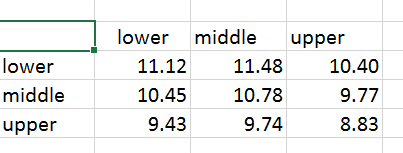
\includegraphics[width=8cm]{10-5-6-a.png}
  \caption{$R_iC_j$ table}
  \label{fig:boat1}
\end{figure}


\begin{figure}[h!]
\centering
  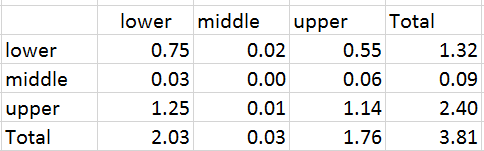
\includegraphics[width=8cm]{10-5-6-b.png}
  \caption{$d_1$'s table}
  \label{fig:boat1}
\end{figure}

\end{document}


\section{Tables}
\begin{figure}[h!]
  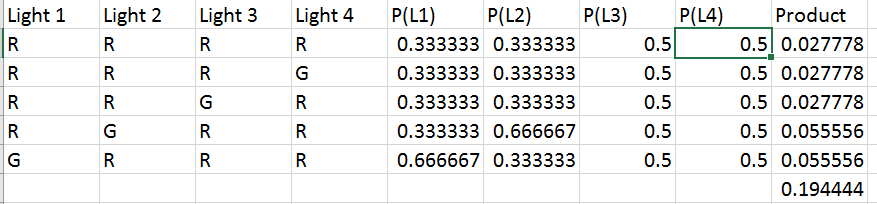
\includegraphics[width=\linewidth]{2-5-16.png}
  \caption{Excel table for 2-5-16}
  \label{fig:boat1}

https://wolfweb.unr.edu/~drschmidt/stat467hw8sln.pdf
http://jekyll.math.byuh.edu/courses/m321/handouts/gammahalf.pdf
https://studylib.net/doc/18411298/proof-of-gamma-1-2-

https://wolfweb.unr.edu/~drschmidt/stat467hw8sln.pdf
